\chapter{Basic concepts}
\label{basic_concepts}
Spot essentially manipulates $\omega$-automata which is a variation of finite-state automata (FSA) that runs
on infinite, rather than finite. Automata theory crop up preety much everywhere in computer science.
In logic design, natural language processing, system analysis, regular expressions, etc. This
chapter discuss about some basics of automata theory related to $\omega$-automaton and then, the 
satisfiability problem.

\section{Automata theory}
This section consists essentially of excerpts of Spot's \textbf{concept}~\cite{8} and
wikipedia $\omega$-automaton web pages. Feel free to have a look on these pages for further details.\\

\noindent \textit{Automata theory}~\cite{9} is the study of abstract machines and automata, as well as the
computational problems that can be solved using them.

\begin{figure}[H]
 \centering
 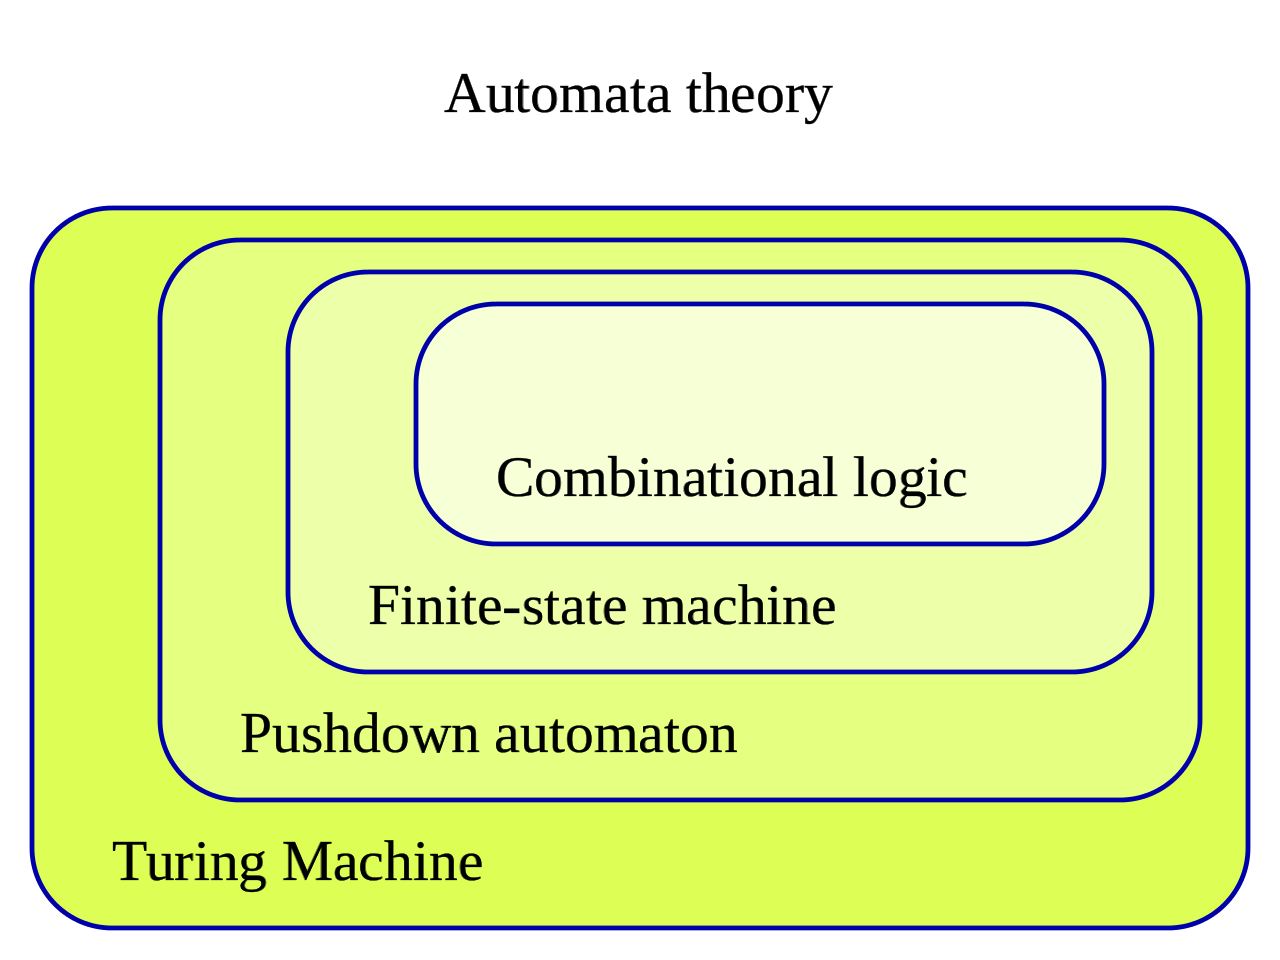
\includegraphics[scale=0.2]{img/automata_classes.png}
 \caption{Classes of finite automata~\cite{9}}
 \label{fig:aut_classes}
\end{figure}
There are different classes of finate automata. The finite state machine has less computational power than
some other models of computation such as the Turing machine~\cite{10}. The computational power distinction
means there are computational tasks that a Turing machine can do but a finite-state automaton (FSA) can
not.\\

\noindent However, the $\omega$-automata would be a simillar but parallal hierarchy.

\subsection{Atomic preposition}
An \textit{atomic proposition} is a named Boolean variable that represents a simple property that must be
true or false. It usually represents some property of a system. They are used to construct temporal logic
formulas~\cite{13} to specify properties of the system.

\subsection{Boolean formula}
A Boolean formula is formed from \textit{atomic preposition}, the Boolean constants true and false, and
standard Boolean operators like and, or, implies, xor, etc.

\subsection{$\omega$-words}
An $\omega$-word is a word of infinite length. In our context, each letter is used to
describe the state of a system at a given time, and the sequence of letters shows the evolution of the
system as the (discrete) time is incremented.\\

If the set \textbf{AP} of atomic propositions is fixed, an $\omega$-word over \textbf{AP} is an infinite
sequence of subsets of \textbf{AP}. In other words, there are 2$^{|\textbf{AP}|}$ possible letters to
choose from, and these letters denote the set of atomic propositions that are true at a given instant.\\

For instance if \textbf{AP}$=\{a,b,c\}$, the infinite sequence $\{a,b\}$;$\{a\}$;$\{a,b\}$;$\{a\}$;
$\{a,b\}$;$\{a\}$;… is an example of $\omega$-word over \textbf{AP}. This particular $\omega$-word can be
interpreted as the following scenario: atomic proposition $a$ is always true, $b$ is true at each other
instant, and $c$ is always false.

\subsection{$\omega$-Automaton}
An $\omega$-automaton is used to represent sets of $\omega$-word.\\

It is defined by a quintuplet $M=(AP, Q, q_o, X, \alpha)$ where:
\begin{itemize}
 \item $AP$ is a set of Atomic Proposition,
 \item $Q$ is Q is a finite set. The element of $Q$ are called states of $M$,
 \item $Q_0 \subset Q$ is the set of initial states. If the automaton is deterministic, there is only one
       initial state $q_0 \in Q$. Determinism is a notion defined below.
 \item $X$ can be either a transition function $\delta : Q \times 2^{AP} \rightarrow Q$ (if the automaton is
       deterministic) or a transition relation $\Delta \subset (Q \times 2^{AP} \times Q)$ (if it is not
       deterministic). 
 \item And $\alpha$ is a positive Boolean function over terms of the form $Fin(T)$ or $Inf(T)$ with
       $T \subseteq \Delta$. This is also called the \textit{acceptance condition}.
\end{itemize}

The language of an $\omega$-automaton is the set of $\omega$-words it accepts.\\

There are many kinds of $\omega$-automata and they mostly differ by their acceptance condition. The
different types of acceptance condition, and whether the automata are deterministic or not can affect their
expressive power.

\subsection{Determinism}
An automaton is said to be \textit{deterministic} iff for each pair of state and symbol ($Q \times 2^{AP}$)
there is one and only one transition to a next state.\\

\noindent A \textit{non deterministic} automaton allows:
\begin{itemize}
 \item many transitions labeled by the same symbol and outgoing from the same state,
 \item transitions labeled by the \textit{empty word} $\varepsilon$,
 \item transitions labeled by more than one symbol.
\end{itemize}

\noindent Therefore, for each pair of state and symbol, there is no more one destination state but a set of
possible destination states. Hence the $Q \times 2^{AP} \times Q$.

\subsection{$\omega$-Automaton run}
A run of $M$ on the input $(a_1, a_2, a_3,...)$ is any infinite sequence
$\rho = (r_0, r_1, r_2,...)$ of states that satisfies the following conditions:
\begin{itemize}
 \item $r_0$ is an element of $Q_0$,
 \item $r_1$ is an element of $\Delta(r_0, a_1)$,
 \item $r_2$ is an element of $\Delta(r_0, a_2)$.\\...
 \item $r_n$ is an element of $\Delta(r_{n-1}, a_n)$,
\end{itemize}

A nondeterministic $\omega$-automaton may admit many different runs on any given input, or none at all.
The input is accepted if at least one of the possible runs is accepting. Whether a run is accepting depends
only on $\alpha$, as for deterministic $\omega$-automata. Every deterministic $\omega$-automaton can be
regarded as a nondeterministic $\omega$-automaton by taking $\Delta$ to be the graph of $\delta$.
The definitions of runs and acceptance for deterministic $\omega$-automata are then special cases of the
nondeterministic cases.

\subsection{Transition-based vs. State-based acceptance}
The figure~\ref{fig:omega_aut} has state-based acceptance set, runs are accepting if these visit infinitely
often some state in each acceptance set, etc. Transition-based acceptance means acceptance sets are now
sets of transitions and runs are accepting if the transitions they visit satisfy the acceptance condition.\\

Using transition based acceptance allows fore more compact automata. Here is two representations of the
formula $GFa$ (infinitely often a):

\begin{figure}[H]
 \centering
 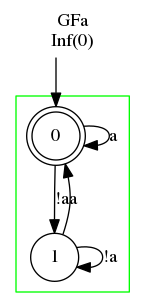
\includegraphics[scale=0.8]{img/state_based.png}
 \caption{State based automaton representing formula \textbf{GFa}}
 \label{fig:state_based}
\end{figure}

\begin{figure}[H]
 \centering
 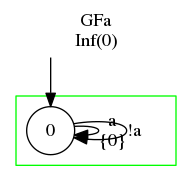
\includegraphics[scale=0.8]{img/trans_based.png}
 \caption{Transition based automaton representing formula \textbf{GFa}}
 \label{fig:transition_based}
\end{figure}

\subsection{Acceptance condition}
An acceptance condition actually consists of two pieces: some acceptance sets, and a formula that tells
how to use these acceptance sets.\\

Acceptance formulas are positive Boolean formula over atoms of the form $t$, $f$, $Inf(n)$, or $Fin(n)$,
where $n$ is a non-negative integer denoting an acceptance set.
\begin{itemize}
 \item $\textbf{t}$ denotes the true acceptance condition: any run is accepting
 \item $\textbf{f}$ denotes the false acceptance condition: no run is accepting
 \item $\textbf{Inf(n)}$ means that a run is accepting if it visits infinitely often the acceptance set n
 \item $\textbf{Fin(n)}$ means that a run is accepting if it visits finitely often the acceptance set n
\end{itemize}

The above atoms can be combined using only the operator $\&$ and $|$ (also known as $\land$ and $\lor$), and
parentheses for grouping. Note that there is no negation, but an acceptance condition can be negated
swapping $t$ and $f$, $\land$ and $\lor$, and $Fin(n)$ and $Inf(n)$.\\

The following table gives an overview of how some classical acceptance condition are encoded. The first
column gives a name that is more human readable (those names are defined in the HOA~\cite{3} format and
are also recognized by Spot). The second column give the encoding as a formula.

\begin{figure}[H]
 \centering
 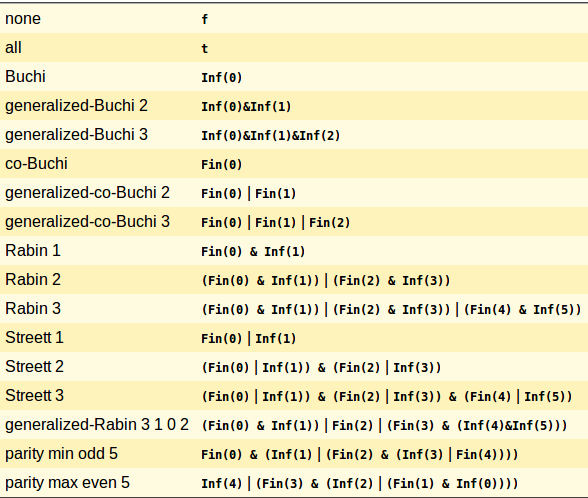
\includegraphics[scale=0.6]{img/acc_conds.png}
 \caption{$\omega$-automata acceptance conditions~\cite{8}}
 \label{fig:acc_conds}
\end{figure}

\subsection{Completeness}
An automaton is said to be complete iff for each pair of state and input, there is at least one transition
to a next state.

\section{SAT solver}
Satisfiability problem is a classic of computer science.\\

The purpose of SAT solving is to assign each variables of a propositional formula in such a way that the
formula evaluates to true. It is the canonical NP-complete problem. SAT solvers are used to solve many
practical problems and this is also the case in Spot, they are used to minimize $\omega$-automata.\\

\subsection{Disjunctive Normal Form (DNF)}
A logical formula is said to be in disjunctive normal form if it is a disjunction of conjunctive clauses.
It can also be described as an OR of ANDS. Note that the \textbf{not} operator $\neg$ is authorized and can
only be used as part of a litteral. For instance, the
following formulas are in DNF:
\begin{itemize}
 \item $(A \land B \land C) \lor (\neg A \land B \land \neg C) \lor (A \land \neg B \land C)$
 \item $A \lor (B \land C)$
 \item $A \lor B \lor \neg C$
\end{itemize}
To solve such a formula, as it is a disjuction of cunjunctive clauses, it can be considered as an
enumeration of possible solutions. Each conjunctive clause is a solution sufficient to evaluate all the DNF
to true.

\subsection{Conjunctive Normal Forms (CNF)}
Similarly, a conjunctive normal form is a logical boolean formula that consists of conjunction of clauses
--- clauses being a disjunction of litterals. it can also be described as an AND of ORS and the operator
$\neg$ is also authorized, only attached to a litteral.
\begin{itemize}
 \item $\neg A \land (B \lor C)$
 \item $(A \lor B \lor C) \land (D \lor \neg E) \land (F)$
 \item $ (A \lor B) \land (\neg A \lor C) $
\end{itemize}
Solving such a formula is not as easy as DNF formulas. SAT solvers can solve these CNF formulas.

\subsection{DIMACS format}
DIMACS is a file format used to define a boolean expression written in conjunctive normal form. This file
can be used as input for SAT solvers --- SAT problems are encoded in a file following DIMACS
format~\cite{18}. For more details, \textbf{SAT-solving in practice}~\cite{16} is a good introduction to
SAT solvers.